\documentclass[12pt]{article}

\usepackage{fullpage}
\usepackage{framed}
\usepackage{standalone}
\usepackage{amsmath}
\usepackage{tikz}

% rename 'part' to 'phase'
\renewcommand{\partname}{Phase}

% command to write requirement
\newcommand{\Requirement}[1] {
   \noindent \textbf{Requirement:} #1
}

% command to write feature
\newcommand{\Feature}[1]{ 
   \noindent \textbf{Feature} #1
}

% command to use template
\newcommand{\CFeature}[4]{
\noindent \textbf{Connextra Feature:}
	\begin{quote}
	\begin{tabular}{rl}
	\textbf{AS A} & #1\\
	\textbf{SO THAT \uppercase{#2}} & #3\\
	\textbf{\uppercase{#2} WANT TO} & #4  
	\end{tabular}
	\end{quote}
}

\newcommand{\GivenSc} {
	\noindent \textbf{GIVEN:}
	}
	
\newcommand{\WhenSc} {
	\noindent \textbf{WHEN:}
	}
	
\newcommand{\AndSc} {
	\noindent \textbf{AND:}
	}
	
\newcommand{\ThenSc} {
	\noindent \textbf{THEN:}
	}

\begin{document}

\documentclass[12pt]{article}

\usepackage{standalone}
\usepackage{fullpage}

% rename 'part' to 'phase'
\renewcommand{\partname}{Phase}

\begin{document}
\part{Project Scoping}
\setcounter{section}{1}
\setcounter{subsection}{0}
\section*{Deliverable 1}
\subsection{GitHub - An Overview}
\textbf{\textsf{GitHub}} is a collaborative site for sharing and working on software projects based around the \textit{Git Version Control System}. It is beneficial when used individually or as a group as it allows for members to use a web-based graphical interface to interact with the command line tool git.\\ 

\noindent \textsf{GitHub}'s advantages are its ability to provide easy interaction between members working on the same project, and its ease of use compared to working from the command line. It allows for easy management of wikis, bug tracking and feature requests.\\

\noindent The \textsf{GitHub} system also contains features for sharing small code snippets (Gists) which act like normal repositories, so that they can be changed by the author (managed by Git version control on the website) and forked (making a separate copy of the project). Contributors are able to make changes to their projects locally and then push their changes to \textsf{GitHub}, but also can make changes directly on the online \textsf{GitHub} service as well.


\setcounter{section}{2}
\setcounter{subsection}{0}
\section*{Deliverable 2}
\subsection{Vision Statement}
To create a website which interfaces with \textsf{GitHub}'s API allowing for a more advanced searching of repositories and improving a user's experience of viewing a project; both in an holistic perspective and a detailed view. We also aim to link relevant sections of code with documentation from the wiki and allow for an easier workflow for the user.
\subsection{General Goals}
\begin{itemize}
\item Expand the \emph{Explore GitHub} page and allow users to search for specific projects to increase contribution with a larger variety of open source projects.
\item Provide and display relevant information and statistics in an intuitive manner to aid users with choosing new open source projects.
\item Construct easy access between code and relevant documentation.
\item Create a simple and convenient way to navigate through documents, files and folders; allowing for users to view and contribute to specific sections easier.
\item Mediate a wider variety of resources (including statistics, code and projects) for utilisation.
\item Create a holistic view of projects to understand how systems interact with one another, allowing for deeper learning in the workings of current and new projects.
\end{itemize}
\subsection{Group/Team Goals}
\textbf{Statistics Team}: (Josh \& Daniel)
\begin{itemize}
\item Gather resources and statistics from current projects hosted on GitHub
\item Working with the \emph{Visual Team} to provide statistics which will shape the UI and workflow.
\end{itemize}
\textbf{Visual Team}: (Sanjay, Robert \& Paul)
\begin{itemize}
\item Develop a seamless User Interface (UI) that flows from the existing, to allow easy access to important data.
\item Creation of shortcuts to speed up common tasks (utilising data supplied from the \emph{Statistics Team}).
\end{itemize}
\subsection{Individual Team Member Goals}
\begin{enumerate}
\item Josh - Browse multiple repositories on \textsf{GitHub} in order to devise a set of statistics which consider a project to be be more readily contributable.
\item Daniel - Develop a system to aid users in selecting a project by displaying relevant statistics such as average input per contributor.  
\item Paul - Develop a visual based system to manage and see the interactions between project files and other projects hosted on \textsf{GitHub}.
\item Sanjay - Implementing methods for connecting functions from user code to the wiki. Also to oversee development of our project documentation using \LaTeX\ .
\item Robert - To provide a more convenient way of viewing code by implementing the collapsing of functions/code blocks.
\end{enumerate}

\pagebreak
\setcounter{section}{3}
\setcounter{subsection}{0}
\section*{Deliverable 3}
\subsection{Problem Statements}
At the current state, \textsf{GitHub}:
\begin{enumerate}
\item  Does not have more advanced searching of repositories to find more readily contributable open source projects.
\item Does not display enough statistics (e.g. Average input per contributor) to aid with choosing a new project.
\item Does not  have a visual way to view a whole project (e.g. how all the classes/files interact, UML diagrams generated from code).
\item Does not link documentation from a repository's wiki with the relevant functions/lines in the project's code.
\item Does not allow functions/blocks of code to be collapsed for easy targeted viewing online.
\end{enumerate}

\subsection{Inference for Problem Statements}
Inference for our problem statements stemmed from previous work and experience with \textsf{GitHub}. With a moderate level of knowledge of \textsf{GitHub}, we were able to identify a lack of features prevalent within usage of the system. Those of us who had lacked experience with usage of \textsf{GitHub} were quick to investigate and understand some important features to be missing.

Our first problem statement was brought up as a way to encourage younger or novice programmers to take part in contribution to open-source projects. Finding and aiding in projects that are large, cumbersome and complex are oft-not viable for programmers starting out in the field. Hence we proposed developing a more refined search feature that allows to find more readily contributable open source projects. Essentially, we would be enhancing resources available for the user.

The lack of a diverse set of statistics (such as average contribution per user) was a driving factor for our second problem statement, complementing our first problem statement. The availability of a greater set of statistical resources would be beneficial to aid individuals in finding suitable projects to work on. This was our inference for our second problem statement.

We also observed, explored and identified the absence of a visual aspect within the \textsf{GitHub} system. We realised the lack of a holistic view of code on \textsf{GitHub}. Previous work with software development prompted us to understand the need for a more visual aspect to viewing the relationships, connections and associations with other files in the repository.

The absence of a link between \textit{code}, (be it the functions within the code or only certain lines of code) and its respective \textit{documentation} was also another feature which we believe would he helpful. Prior work with coding and looking up relevant documentation for a function prompted us to list this fourth problem statement.

Our final statement was also another visual aspect. Once again, due to previous coding experience we realised the ability to collapse sections of code would provide a more pleasing, aesthetic look. As opposed to a large, clumsy, confusing code layout, we believe this feature would allow the end-user to focus their attention on a particular section.

All in all, we derived the essence of our problem statements based upon problems that we had previously encountered. We also formulated the problem statements for features and resources that we believed would enhance the user experience of the \textsf{GitHub} system.

\end{document}


\pagebreak
\setcounter{part}{1}
\setcounter{section}{1}
\setcounter{subsection}{0}
\part{User Stories}
\section*{Deliverable 1}
\subsection{User Stories}


\begin{framed}
\subsubsection{Requirement: Advanced Search}
\noindent A more advanced searching of repositories to find more readily contributable open source projects.\\[0.2cm]

\hrule~\\

\noindent\Feature{\textbf{1:} An advanced search panel for finding repositories that I can commit to.}\\[0.2cm]


\CFeature{user (\textsf{GitHub} contributor)}{I}{can help other developers}{Find repositories that I can contribute to}

\noindent \textbf{Scenario}:
\begin{quote}
\begin{tabular}{rl}
\GivenSc & that I am on the main page\\
%\AndSc & lel\\
\WhenSc & I click on ``Find Repos"\\
\ThenSc & I can see a list of repositories with some basic stats next to each one
\end{tabular}
\end{quote}

\hrule~\\

\noindent\Feature{\textbf{2:} Filter repositories based on a number of parameters.}\\[0.2cm]

\CFeature{user (\textsf{GitHub} contributor)}{I}{can find more relevant repositories}{filter a list of repositories}

\noindent \textbf{Scenario}:
\begin{quote}
\begin{tabular}{rl}
\GivenSc & that I am on the main page\\
%\AndSc & lel\\
\WhenSc & I select some parameters and click on ``Find Repos''\\
\ThenSc & I can see a sorted list of repositories based on my parameters
\end{tabular}
\end{quote}
\end{framed}

\begin{framed}
\subsubsection{Requirement: Diverse set of Statistics}
Display enough statistics to aid with choosing a new project.\\[0.2cm]

\hrule~\\

\noindent\Feature{\textbf{3:} Repositories lists the average amount of commits per contributor}\\[0.2cm]

\CFeature{User (\textsf{GitHub} contributor)}{I}{Can view other contributors motivation}{Pick a repository that has high contribution rates}

\noindent \textbf{Scenario}:
\begin{quote}
\begin{tabular}{rl}
\GivenSc & that I am viewing a repository's statistics\\
%\AndSc & lel\\
\WhenSc & I click on ``Contributors"\\
\ThenSc & I can view the average commits per contributor
\end{tabular}
\end{quote}

\hrule~\\

\Feature{\textbf{4:} Repositories graphs average consecutive days for commits from contributors}\\[0.4cm]

\CFeature{User (\textsf{GitHub} contributor)}{I}{Know frequently I need to contribute}{View how frequently commits are made by contributors}

\noindent \textbf{Scenario}:
\begin{quote}
\begin{tabular}{rl}
\GivenSc & that I am viewing a repository's statistics\\
%\AndSc & lel\\
\WhenSc & I click on ``Loyalty"\\
\ThenSc & I can see whether other contributors stay long
\end{tabular}
\end{quote}
\end{framed}

\pagebreak
\begin{framed}
%%% TEMPLATE %%%
% Requirement (problem statement)
\subsubsection{Requirement: Link to Code's Documentation}
Link documentation from a repository's wiki with the relevant functions/lines in the project's code.\\[0.2cm]

\hrule~\\

% Feature
\noindent \Feature{\textbf{5:} Code in repository opens a hyperlink to the complete wiki documentation.}\\[0.2cm]

% Feature
\noindent \textbf{Connextra Feature}:
\begin{quote}
\begin{tabular}{rl}
\textbf{AS A}      & Code viewer\\
\textbf{SO THAT I} & understand the inner-workings of raw code.\\
\textbf{I WANT TO} & read the explanation for written code
\end{tabular}
\end{quote}


% Scenario
\noindent \textbf{Scenario}:
\begin{quote}
\begin{tabular}{rl}
\GivenSc & that I am viewing raw code in a repository\\
\WhenSc & I click on a function\\
\ThenSc & I should be linked to specific section of wiki explaining the code. 
\end{tabular}
\end{quote}


% Feature - GitHub contributor
\noindent \textbf{Connextra Feature}:
\begin{quote}
\begin{tabular}{rl}
\textbf{AS A}      & \textsf{GitHub} contributor\\
\textbf{SO THAT I} & can help new users understand the inner-workings \\
                   & of raw code.\\
\textbf{I WANT TO} & set up a hyperlink for code viewers to understand my\\
                   &  written code.
\end{tabular}
\end{quote}

% Scenario
\noindent \textbf{Scenario}:
\begin{quote}
\begin{tabular}{rl}
\GivenSc & that I am developing a wiki documentation\\
\WhenSc & I click on ``Connect Code to Wiki''\\
\AndSc & I specify which line I want to connect to\\
\ThenSc & I should be able to set up a hyperlink to the wiki documentation.
\end{tabular}
\end{quote}

\hrule~\\

\noindent \Feature{\textbf{6:} A small tool tip summary of that data type is shown (showing its methods and attributes.)}\\[0.2cm]

% Feature
\noindent \textbf{Connextra Feature}:
\begin{quote}
\begin{tabular}{rl}
\textbf{AS A}      & Code viewer\\
\textbf{SO THAT I} & understand the implementation of data types in written code.\\
\textbf{I WANT TO} & see the data type's methods \& attributes
\end{tabular}
\end{quote}

\pagebreak
% Scenario
\noindent \textbf{Scenario}:
\begin{quote}
\begin{tabular}{rl}
\GivenSc & I am observing the data type in the code\\
\WhenSc & I hover my mouse over a data structure\\
\ThenSc & a tool-tip window show display, showing the \\ 
        & attributes and methods of the data type.
\end{tabular}
\end{quote}

% Feature - GitHub contributor
\noindent \textbf{Connextra Feature}:
\begin{quote}
\begin{tabular}{rl}
\textbf{AS A}      & \textsf{GitHub} contributor\\
\textbf{SO THAT I} & I possess the tools to develop a tool-tip activated \\                    
                   & by mouse hover\\
\textbf{I WANT TO} & construct a way for users to posses a greater understanding \\
                   & of data structures in code.
\end{tabular}
\end{quote}

% Scenario
\noindent \textbf{Scenario}:
\begin{quote}
\begin{tabular}{rl}
\GivenSc & I am developing a wiki documentation\\
\WhenSc & I click on ``Make Tool-Tip''\\
\AndSc &  I specify which data structure I want to connect to\\
\ThenSc & I should be able to develop a tool-tip explaining methods\\
        &  \& attributes of the data structure.
\end{tabular}
\end{quote}
\end{framed}

% PAUL
\pagebreak
\begin{framed}
\subsubsection{Requirement: Visual View of Project}
A visual way to view a whole project.\\[0.2cm]

\hrule~\\

\noindent \Feature{\textbf{7:} Diagrams based on how files interact with one another}\\[0.2cm]

% Feature
\noindent \textbf{Connextra Feature}:
\begin{quote}
\begin{tabular}{rl}
\textbf{AS A}      & user (\textsf{GitHub} contributor)\\
\textbf{SO THAT I} & can gain a deeper understanding of how the project\\
                   & utilises other projects.\\
\textbf{I WANT TO} & Find more projects linked to the current project.
\end{tabular}
\end{quote}

% Scenario
\noindent \textbf{Scenario}:
\begin{quote}
\begin{tabular}{rl}
\GivenSc & that I am viewing a project or file\\
\WhenSc & I click on “Model”\\
\ThenSc & I can get a diagram of which files utilise each other.\\
\AndSc & I can click on the files to open them in a new window.
\end{tabular}
\end{quote}

\hrule~\\

\noindent \Feature{\textbf{8:} Holistic view of functions of code.}\\[0.2cm]

\noindent \CFeature{User (\textsf{GitHub} contributor)}{I}{can easily understand how a file works.}{get a simplified version of the current code.}

% Scenario
\noindent \textbf{Scenario}:
\begin{quote}
\begin{tabular}{rl}
\GivenSc & that I am viewing a file\\
\WhenSc & I click on ``Collapse'' next to a line of code\\
\ThenSc & the code inside the function is hidden.\\
\AndSc & is replaced with arrows showing where the function links to\\
\WhenSc & I click on ``Collapse All''\\
\ThenSc & the code inside all functions are hidden\\
\AndSc & are replaced with a list using arrows to show where functions link to
\end{tabular}
\end{quote}
\end{framed}

\pagebreak
\begin{framed}
% ###########   ROBERT   ########### 
\subsubsection{Requirement: Statistics based Contributor Search}
The ability to search for users (contributors) based on how active they are and what kind of projects they contribute to.\\[0.2cm]

\hrule~\\

\noindent \Feature{\textbf{9:} Searching for users based on how active they are.}\\[0.2cm]

% Feature
\noindent \textbf{Connextra Feature}:
\begin{quote}
\begin{tabular}{rl}
\textbf{AS A}      & User (\textsf{GitHub} author)\\
\textbf{SO THAT I} & can collaborate with more active users\\
\textbf{I WANT TO} & be able to search for users based on their average contributions
\end{tabular}
\end{quote}

% Scenario
\noindent \textbf{Scenario}:
\begin{quote}
\begin{tabular}{rl}
\GivenSc & that I am on the main page\\
\WhenSc  & I click on ``Find Users"\\
\AndSc   & I select the parameter "Sort by User Activity" and click ``Search"\\
\ThenSc  & I can see a filtered list of users based on their average \\ 
         & daily/weekly contributions 
\end{tabular}
\end{quote}

\hrule~\\

\noindent \Feature{\textbf{10:} Searching for users based on what kind of projects they contribute to.}\\[0.2cm]

% CFeature
\noindent \textbf{Connextra Feature}:
\begin{quote}
\begin{tabular}{rl}
\textbf{AS A}      & User (\textsf{GitHub} author)\\
\textbf{SO THAT I} & can collaborate with users who have similar interests\\
\textbf{I WANT TO} & be able to search for users based on the type of projects \\
                   & they've contributed to.
\end{tabular}
\end{quote}

% Scenario
\noindent \textbf{Scenario}:
\begin{quote}
\begin{tabular}{rl}
\GivenSc & that I am on the main page\\
\WhenSc  & I click on ``Find Users"\\
\ThenSc  & I can open up the ``Advanced Search"\\
\WhenSc  & I select one of the project types under the ``Project Categories"\\
         & subheading\\ 
\AndSc   & I click ``Search"\\
\ThenSc  & I can see a list of users who have contributed to any projects \\
         & of the relevant type
\end{tabular}
\end{quote}

\pagebreak

% ROBERT'S NEW SUB-FEATURE
\noindent \Feature{\textbf{11:} Users can sort their projects/repositories according to category.}\\[0.2cm]

% CFeature
\noindent \textbf{Connextra Feature}:
\begin{quote}
\begin{tabular}{rl}
\textbf{AS A}      & \textsf{Github} author\\
\textbf{SO THAT I} & have an alternative to sorting my projects\\
\textbf{I WANT TO} & be able to sort my projects by their category \\
\end{tabular}
\end{quote}


% Scenario
\noindent \textbf{Scenario}:
\begin{quote}
\begin{tabular}{rl}
\GivenSc & that I am viewing my own \textsf{Github} profile\\
\WhenSc  & I click on the ``Repositories" tab\\
\AndSc   & I click on ``New"\\
\ThenSc  & there should a "Category" heading under the description text box\\
\AndSc   & I should be able to select a project category from the list
\end{tabular}
\end{quote}

% Scenario
\noindent \textbf{Scenario}:
\begin{quote}
\begin{tabular}{rl}
\GivenSc & that I am viewing my \textsf{Github} profile\\
\WhenSc  & I click on the ``Repositories" tab\\
\ThenSc  & I can open up the ``Advanced Search"\\
\WhenSc  & I select ``Sort by project category"\\
\AndSc   & I click ``Search"\\
\ThenSc  & I can see my projects sorted into columns\\ 
         & (one column for each project type)
\end{tabular}
\end{quote}
\end{framed}

\pagebreak
\documentclass[12pt]{article}

\usepackage{fullpage}
\usepackage{framed}
\usepackage{standalone}
\usepackage{amsmath}
\usepackage{tikz}

\begin{document}
\part*{Glossary}
\begin{table}[!htb]
\begin{tabular}{rl}
\noindent \textbf{Method}   & a group of commands grouped together to perform an operation (like a `function')\\
                             & \\
\noindent \textbf{Tool-Tip} & a small message which appears when a cursor is positioned over an image,\\
                             &  text or hyperlink.\\
                             & \hfill 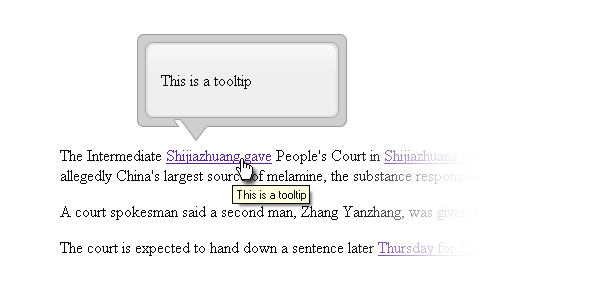
\includegraphics[scale=0.7]{tooltip}\\
                             & \\
                             & \\
                             & \\
                             & \\
                             & \\
                             & \\
\end{tabular}
\end{table}
\end{document}

\end{document}
